\section{Introduction}

Ever-increasing data collection capabilities (such as genomic sequencing, telemetry studies of animal behaviour, or remote sensing of environmental variables), in combination with large-scale synthesis of existing data bases on species occurrence and phenotypic traits, are making large volumes of biological data available over an ever-wider taxonomic range.
As a result, researchers are interested in exploring ways to study more complicated systems and fitting more models to data or synthetic databases of species traits.
One particular area of growth is phylogenetic comparative analysis using phylogenetic (eco-evolutionary) regression \cite{hansen2012interpreting}. 
Comparative analyses explore the relationships among species traits (including occurrence within communities) while taking the underlying/latent evolutionary relationships of the species into account; in some cases, researchers are interested in quantifying the evolutionary signals underly traits rather than simply controlling for them.
Unlike ordinary regression, where biologist look at the change in the of predictor variables (for example, species trait and environmental factors) on the response variable that are often observable; in phylogenetic regression, the evolutionary relationship between species are unobservable and assumed to evolve in some underlying evolutionary process \citep{felsenstein1985phylogenies, butler2004phylogenetic}. 
While evolutionary relationships are biologically important and interesting, they often get neglected in multi-species analyses. 
Recently, biologist have started to incorportate phylogenetic relationships to multi-species modelling, and there exist a range of statistical tools for comparative analyses, but many of these tools are either inflexible, or too computationally expensive to analyze large volumes of data.
In such cases, researchers may try to find ways to simplify their analyses (i.e. simplifying the model by making assumptions of the evolutionary process) \citep{bunnefeld2012island, ord2010adaptation},
%% bunnefeld2012island: used taxon for random slopes but did not include phylogenetic information
%% ord2010adaptation : used OU process with means (single obs per taxa),
%%  i.e. ignoring within-taxon variation?
which can lead to statistical issues and erroneous conclusions
\cite{felsenstein1985phylogenies, li2017statistical}.
% \bmb{What precise ``issues'' do you have in mind? Don't think we need to state them here, but we should know. Based on your comments, I can guess that (1) by using random slopes across taxa, Bunnefeld 2012 is neglecting more subtle variation due to differential relatedness? (2) not sure whether taking taxon-level means (Ord 2010) is actually a problem. Ignores some variation,
% but it might be ignorable (cf. Murtaugh 2007 ``Simplicity and complexity in ecological data analysis'')}
In this paper, we propose an alternative method for flexibly and efficiently modeling phylogenetic relationships via mixed effect models, highlighting various complexities of phylogenetic relationships through random effects.
% \bmb{nice!}

There are two general challenges in linking the evolutionary process to a phylogenetic comparative statistical framework.
% Phylogenetic signal : the magnitude of phylogenetic correlation
The first challenge is to identify and segregate phylogenetic signals \citep{blomberg2003testing} and other sources of variation that are present in residuals.  
% \bmb{prev sentence doesn't seem be quite the right lead-in to the rest of the paragraph? You go on to talk about the tip-variation/residual-variation confounding issue. Maybe replace with something talking more specifically about resolving tip variation?}
The classic phylogenetic regression assumes that phylogenetic correlation (PC) among the residuals from a regression between the traits arises because the residual variation evolves along the branches of the phylogeny according to a Brownian motion process; if the traits are normally distributed and observed without any additional error or within-species variation, this leads to Felsenstein's method of phylogenetically independent contrasts (PICs) \citep{felsenstein1985phylogenies}.
More recent approaches -- including phylogenetic generalized linear mixed models (PGLMM) \citep{ives2011generalized}, Pagel's $\lambda$ \citep{pagel1999inferring}, and Blomberg's $K$ \citep{blomberg2003testing} --- build upon Felsenstein's PICs by considering different response distributions and allowing extra parameters to account for additional complexities in the evolutionary process. They partition the phylogenetically correlated residual variation into (1) phylogenetically uncorrelated residual variation (observation error or tip variation) and (2) phylogenetic signal  \citep[biological/evolutionary process error:][]{hansen2012interpreting}.
However, when multiple observations (or repeated measures) of the same species (taxon) are being observed, this introduces another level of variation; in this case, phylogenetic signal and tip variation are now both part of the evolutionary process error (we will call this species/intercept level variation) and residual variation is associated with observation level variation (the standard statistical definition).
\mli{See shiny}
%\bmb{This is a good point, well expressed. Does PGLMM lump tip variation and within-species variation, or is this primarily an issue with Blomberg/Pagel? Thinking about Boettiger's critique \cite{boettiger2013is} (don't know if it's been peer-reviewed, we could ask him), which might be resolved if we think explicitly about within-species variation \ldots
%\mli{I think it is more like our simulation test. In Boettiger's example, it is treating sister taxa as different species. So it is using a phylogenetic tree of 8 species instead of 4.}
Despite the addition of multiple observations per tip taxon (species) being statistically straightforward, it is rarely seen: existing platforms are unable to fit multiple observations, or unbalanced design data, or both.
% \bmb{OK, but we should be prepared to support this. Could we construct a table of existing approaches/platforms with their capabilities?}


The second challenge is flexibly model phylogenetic relationships to other predictor variables (predictor level variation), that is, the variation among multiple different grouping predictor variables (random levels) or variation in effects (random slopes) (i.e phylogenetically related species may behave/ have similar changes in effect or in similar conditions) as well as correlated variation.
While it is reasonable to examine evolutionary relationships between species with their response, it is plausiable the changes in effect or levels of the predictor variables have on the response variable are also phylogenetically correlated. 
%\bmb{maybe we can focus on random slopes here? Need to point out that example studies below are \emph{exceptions} to the general assumption of random intercepts only (how did they manage to do their inference?)}
Several recent studies have tried to incorporate phylogenetic signals beyond species level and looked at species response to phylogenetic signals with changes in environmental factors.
For example, \cite{nowakowski2018phylogenetic} considered phylogenetically correlated slopes in response to habitat conversion when studying the abundance of amphibian species, while \cite{li2017canfun} considered phylogenetically correlated species nested within sites for plant abundance. 
The tools available for extending phylogenetic relationships to predictor variables (or predictor level variation) are relatively inflexible; thus, sophisticated biologists have turned to more flexible Bayesian approaches, despite their computational burden \cite{hadfield2010mcmc, burkner2016brms}.
Table 1 provides a summary of model complexities, platforms and data constraints for phylogenetic comparative analysis.

\newcommand{\pkg}[1]{{\tt #1}}
\newcommand{\code}[1]{{\tt #1}}

\begin{tabularx}{\textwidth}{|X|X|X|X|}
\hline
Model & Method & Data & Platform \\
\hline
\hline
GLM (Simple)  & No Residual & Single Observation & GLS \\
\hline
              & Residual    & Single Observation & Pagel's $\lambda$ \\
              & + phylo intercept &                    & Blomberg's $K$ \\ 
              &             &                    & phylolm \\
\hline
GLMM (Complex)& Random effects & Single Observation & \pkg{pez} \\ 
              &                & Balanced Design &  \\
\hline
              &                & Unrestricted  & \pkg{lme4}, \pkg{glmmTMB} \\
\hline
Bayesian GLMM &                & Balanced Design & \pkg{MCMCglmm} \\ 
\hline        
              &                & Unrestricted   & \pkg{brms} \\
\hline
\end{tabularx}


In this paper, we will propose an alternative formulation of phylogenetic generalized linear mixed models that is mathematically equivalent to previous approaches.
Our new formulation is more flexible; it can be incorporated relatively easily into any mixed-model platform that allows new random-effects design matrices to be specified, and can be easily extended along with the features of mixed model such as multiple observational designs, phylogenetic random-slopes models, and multiple (nested or crossed) random effects.
We will compare our technique coded in R package \pkg{lme4} and \pkg{glmmTMB} with existing methods/platforms (i.e. \pkg{nlme} \citep{pinheiro2014r}, \pkg{phylolm} \citep{ho2014phylolm}, \pkg{pez} \citep{pearse2015pez}, \pkg{MCMCglmm} \cite{hadfield2010mcmc}, and \pkg{brms} \citep{burkner2016brms}) to data from simulated model that incorportates phylogenetic signal from both predictors and tips/species, as well as residual variation.
In principle, for any given valid method that matches the simulation model should eventually converge to the simulated parameters. 
We end by discussing opportunities and practicalities of our method and comments on the state of art for this area of research. 

\section{Materials and Methods}

\newcommand{\bX}{{\mathbf X}}
\newcommand{\bbeta}{{\boldsymbol \beta}}
\newcommand{\bmu}{{\boldsymbol \mu}}
\newcommand{\bY}{{\mathbf Y}}
\newcommand{\bC}{{\mathbf C}}
\newcommand{\bZ}{{\mathbf Z}}
\newcommand{\bb}{{\mathbf b}}
\newcommand{\bSigma}{{\boldsymbol \Sigma}}

The typical phylogenetic regression is of the form 

%\bmb{boldface matrices/vectors i.e. $\bX \bbeta$? or not worth the trouble? How about $\bmu=\bX \bbeta$; $\bY \sim \textrm{MVN}(\bmu,\sigma^2 \bC)$ for greater generality? (OK, I see that you move in this direction later.  But I'm not sure it's worth the detour of using two different notations? even if you are going to extend to include fixed effects, $Z$, etc. later ...}:

\begin{align}
\bmu & = \bX \bbeta  \label{eq:gls1} \\ 
\bY & \sim \textrm{MVN}(\bmu,\sigma^{2} \bC), \label{eq:gls2}
\end{align}

where $\bX$ is an $n \times m$ model matrix containing $m$ predictor variables (phenotypic traits or environmental variables, typically including an intercept column of ones); $\bbeta$ is an $m$-vector of coefficients; $\bY$ is an $n \times 1$ response vector and assumed to be multivariate normally distributed with mean $\bmu$ and a variance-covariance matrix given by $\sigma^{2} \bC$ where $\bC$ is a $n \times n$ phylogenetic correlation matrix.
The PC matrix is inferred from the topology of the evolutionary tree by capturing the evolutionary changes that occurred on all the branches, which can be incorporated in statistical methods \citep{garamszegi2014modern}.

%\bmb{give a ref for this? maybe Paradis's ape book, or Garamszegi's book, or ?}
%\mli{chapter 7 in garamszegi 2014}

% More recently, researchers use linear mixed model and generalized linear mixed model framework to model complex systems with phylogenetic structures.
%\mli{Why? Data type, interactions, random effects, etc... Need to really explain random effects here. Alternatively, we can drop this line and write this...}
An alternative modelling approach is to use linear mixed effects modelling framework \citep{lynch1991methods}.
The typical linear mixed model has the form:
\begin{align}
\bY & \sim \textrm{Distr}(\bmu) \label{eq:glmm1} \\
g(\bmu) & = \bX \bbeta + \bZ \bb \label{eq:glmm2} \\
\bb & \sim \textrm{MVN}(0, \bSigma(\theta)) \label{eq:glmm3}
\end{align}
where $Z$ is an $n \times m$ model matrix for the $m$ -- dimensional vector-valued $m$ predictor variables; $\bb$ is the conditional modes and assumed to be multivariate normally distributed with a variance-covariance matrix given by $\bSigma(\theta)$.
Analogously, the phylogenetic regression given by \ref{eq:gls1} can be represented in the mixed model framework by constraining $\bSigma(\theta) = \sigma^2 \bC$.

\bmb{worth including the \pkg{MCMCglmm}/\pkg{brms} inverse-VCV formulation here? And/or contacting Eric Pedersen to find out about his Markov Random Field phylog. stuff in GAM?}
\mli{inverse VCV for BLUP? an alternative way to find the inverse of the vcv(phy)}

\subsection{Reformulating phylogenetic covariance matrix}
% The standard problem of phylogenetic comparative methods is to analyze relationships among data where the observations are gathered from nodes (usually tips) of a phylogenetic tree.
% Phylogenetic independent contrasts is a generalization of the paired comparisons method where contrasts are taken for each bifurcation (nodes) in a phylogenetic tree. 
% Assuming that traits evolve independently in each lineage following speciation, then the trait divergences that occur at one node are independent of divergence at other nodes.  


\newcommand{\bS}{{\mathbf S}}
\newcommand{\bJ}{{\mathbf J}}
\newcommand{\bB}{{\mathbf B}}
\newcommand{\bBadj}{{\mathbf B}_{\mbox{\tiny adj}}}
\newcommand{\bomega}{{\boldsymbol \omega}}
\newcommand{\bell}{{\boldsymbol \ell}}
\newcommand{\e}{{ \epsilon}}

An alternative approach is to model the phylogenetic correlation as a \textit{Gaussian process}. 
In particular, suppose that the evolutionary process is a Brownian motion, which means the evolution of a continuous trait is a random walk and daughter species after speciation are all independent.  
In that case, the phylogenetic variability of a particular observation can be written as the sum of the evolutionary changes that occurred on all of the branches in the phylogeny in its past. 
Thus, the evolutionary history for each species can be modeled with a sequence of independent errors with species--branch matrix $\bS$, rather than having to impose a correlation $\bC$.
For example, figure \ref{fig:tree} is a phylogenetic tree with three species, the corresponding $\bS$ is in the form:

\begin{center}
\begin{figure}[h]
  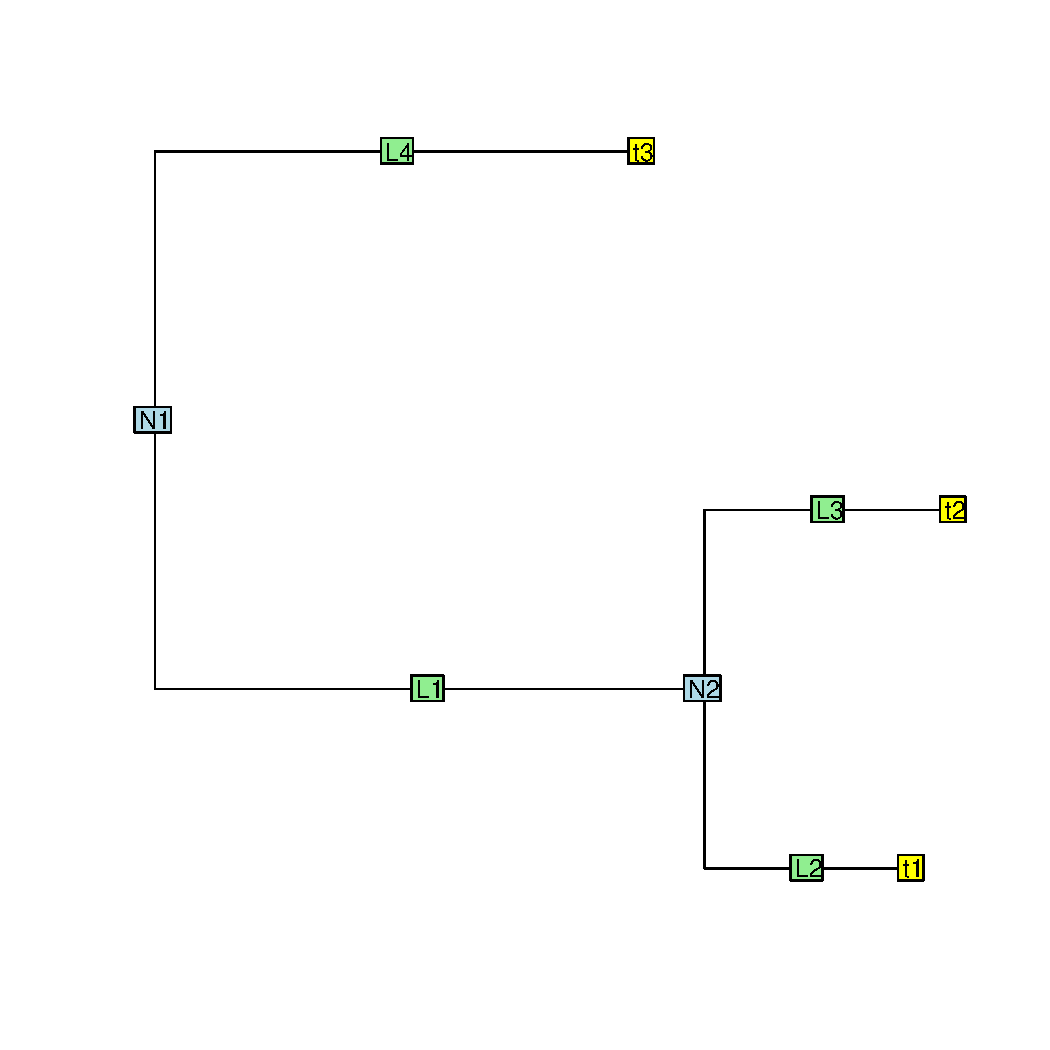
\includegraphics[scale=0.8,page=1]{./git_push/tree.pdf}
  \caption{\bmb{caption ??}}
\label{fig:tree}
\end{figure}
\end{center}

\begin{align*}
\bS = \begin{bmatrix}
\ell_1 \e_1 & \ell_2 \e_2 & 0 & 0 \\
\ell_1 \e_1 &  0 & \ell_3 \e_3 & 0 \\
0  &  0 & 0  & \ell_4 \e_4
\end{bmatrix}
\end{align*}
The error value corresponding to tip 1 is $\ell_1 \e_1 + \ell_2 \e_2$, where $\ell_i$ is the square root of the branch length and the $\ell_i$ are independent, homoscedastic Normal variates. 


\subsubsection*{Constructing the species--branch random effects model matrix}

The error-free $\bS$ is a matrix product of an $n \times b$ indicator matrix $\bS_{ind}$ of branch indices, and a branch length vector $\bell$.

\begin{align}
\bS_{ind} = \begin{bmatrix}
1 & 1 & 0 & 0 \\ 
1 & 0 & 1 & 0 \\ 
0 & 0 & 0 & 1
\end{bmatrix} , 
\bell = \begin{bmatrix}
\ell_1 \\
\ell_2 \\
\ell_3 \\
\ell_4 
\end{bmatrix}
\label{eq:S}
\end{align}
The $\bS$ matrix has a very nice property that $\bS \bS^T$ gives the variance-covariance matrix of the phylogeny. 

The random-effect model matrix $\bZ$ can be decomposed into term-wise model matrix $\bZ_{i}$ as described in \citet{bates2015fitting}.
Thus, the phylogenetic correlated random-effect matrix $\bZ^{C}_{i}$ is

\begin{equation}
\bZ^{C}_{i} = (\bS^{T}_{i}\bJ^{T}_{i} \ast \bX^{T}_{i})^{T}, \label{eq:ZC}
\end{equation}
where $\ast$ is the Khatri-Rao product \citep{khatri1968solutions}, $\bS_{i}$ is an $m_{i} \times b_{i}$ matrix of the species--branch matrix; $\bJ_{i}$ the indicator matrix of grouping factors indices matrix size $n \times m_{i}$; $X_{i}$ is the raw random effects model matrix size $n \times p_{i}$. 


\mli{move example to the supp}
% For example, using the phylogeny above (figure \ref{fig:tree}), if we begin with a raw model matrix,
% 
% \begin{align}
% \bX = \begin{bmatrix}
% 1 & t_1  \\ 
% 1 & t_2  \\ 
% 1 & t_3 
% \end{bmatrix} 
% \end{align}
% then the term-wise phylogenetic random effects model matrix is,
% 
% \begin{align}
% \bZ^{C}_{i} = (\bS^{T}_{adji}\bJ^{T}_{i} \ast \bX^{T}_{i})^{T} =
% \Bigg[
% \Bigg(
% \begin{bmatrix}
% \ell_{adj1} & \ell_{adj1}  & 0 \\
% \ell_{adj2} &  0  & 0 \\
% 0  &  \ell_{adj3} & 0 \\
% 0 & 0 &  \ell_{adj4} 
% \end{bmatrix}
% \begin{bmatrix}
% 1 & 0  & 0 \\
% 0 & 1  & 0 \\
% 0 & 0  & 1  
% \end{bmatrix}
% \Bigg)
% \ast
% \begin{bmatrix}
% 1   & 1   & 1  \\ 
% t_1 & t_2 & t_3
% \end{bmatrix} 
% \Bigg]^T
% \\
% = \begin{bmatrix}
% \ell_{adj1} & \ell_{adj1}t_1 & \ell_{adj2} & \ell_{adj2}t_1 & 0 & 0 & 0 & 0 \\
% \ell_{adj1} & \ell_{adj1}t_2 & 0 & 0 & \ell_{adj3} & \ell_{adj3}t_2 & 0 & 0 \\
% 0 & 0 & 0 & 0 & 0 & 0 & \ell_{adj4} & \ell_{adj4}t_3
% \end{bmatrix}
% \end{align}


% 
% The scaled species--branch matrix $\bS_{adji}$ is scaled version of $\bS$ via the standardized generalized variance (SGV).
% SGVs are used as an intrinsic/natural way to scale down the variance-covariance matrix measured in different scales (for example, phylogenetic distance, years and etc) compariable to other variation in the model \citep{sengupta1987tests}.
% SGV is the $nth$ root of the generalized variance (GV), or the determinant of the variance-covariance matrix, where GV measures the overall size or volume of the variance-covariance matrix.  
% The SGV is given by:
% \begin{align}
% \bomega & = \textrm{det}(\bSigma_{phy})^{1/n},
% \end{align}
% where $n$ is the number of species in the phylogeny.
% 
% The analog in the $\bS$ is to scale the branch vector $\bell$ by square root of the SGV:
% \begin{align}
% \bell_{adj} & = \frac{\bell}{\sqrt{\bomega}}
% \end{align} 
% and the $\bS_{adj}$ is the matrix product of $\bS_{ind}$ and $\bell_{adj}$.

\subsection{Simulation}

We generated test data based on the simple mixed model formulation \ref{eq:glmm1}, \ref{eq:glmm2}, \ref{eq:glmm3} with a single response variable $\bY$ and a single predictor continuous variable $\bX$ for $n$ (25, 50, and 100) species.
For wider range of comparisons, we simulate one observation ($X_i,Y_i$) per species.
For single-site model, the full simulation model is the following:
\begin{align}
\bY & = (\beta_0 + b_{phy_{int}}) + (\beta_1 + b_{phy_{slope}}) X + b_{obs}\\
(b_{phy_{int}}, b_{phy_{slope}}) & \sim \textrm{MVN} \Bigg( 0, \begin{bmatrix}
\sigma^2_{phy_{int}} & \sigma_{phy_{int},phy_{slope}} \\ 
\sigma_{phy_{int},phy_{slope}} & \sigma^2_{phy_{slope}}
\end{bmatrix}
\Bigg) \\
b_{obs} & \sim \textrm{MVN} ( 0 , \Sigma)
\end{align}
where it contains two fixed effect parameters ($\beta_0$ and $\beta_1$), three random effect parameters (phylogenetic random intercept, phylogenetic random slope and correlation between phylogenetic random slope and intercept) and observation/residual variance.  
Predictor and intercept level random variation/effect of species are not applicable in this simulation setting with single observation per species because it will confound with the observational level variation (residuals).

We extend the simulation model by adding multiple sites where each site will have one observation per species. The multiple-site full model is the following: 
\begin{align}
\bY & = (\beta_0 + b_{phy_{int}} + b_{sp_{int}} + b_{site}) + (\beta_1 + b_{phy_{slope}} + b_{sp_{slope}}) X + b_{sp:site} + b_{obs}\\
(b_{phy_{int}}, b_{phy_{slope}}) & \sim \textrm{MVN} \Bigg( 0, \begin{bmatrix}
\sigma^2_{phy_{int}} & \sigma_{phy_{int},phy_{slope}} \\ 
\sigma_{phy_{int},phy_{slope}} & \sigma^2_{phy_{slope}}
\end{bmatrix}
\Bigg) \\
(b_{sp_{int}}, b_{sp_{slope}}) & \sim \textrm{MVN} \Bigg( 0, \begin{bmatrix}
\sigma^2_{sp_{int}} & \sigma_{sp_{int},sp_{slope}} \\ 
\sigma_{sp_{int},sp_{slope}} & \sigma^2_{sp_{slope}}
\end{bmatrix}
\Bigg) \\
b_{site} & \sim \textrm{MVN} ( 0 , \Sigma_{site}) \\
b_{sp:site} & \sim \textrm{MVN} (0, \textrm{Kron}(\bf{I}_{site}, \sigma^2_{phy})) \\
b_{obs} & \sim \textrm{MVN} ( 0 , \Sigma)
\end{align}
The multiple-site full simulation model will have five additional random effects (predictor and intercept level random effect of species and their correlation, random intercept of site and random intercept of species site interaction) compared to the single-site full model.
Predictor and intercept level random effect of species are now applicable in the multiple-site model because there are multiple (one in every site) observations per species. 
Random intercept of species and site interactions is an equivalent version of nested random effects or phylogenetic attraction described in \cite{helmus2007separating} with the main random effects.

\subsection{Platforms}

Our algorithmic approach is general and could be implemented in a wide range of computational platforms that support independent latent variables. 
We implemented our approach using the R packages \pkg{lme4} \citep{bates2015fitting} and \pkg{glmmTMB} \mli{citation}.
We compare our approach with five other R packages that can fit phylogenetic comparative models: \pkg{nlme} \citep{pinheiro2014r}, \pkg{phylolm} \citep{ho2014phylolm}, \pkg{pez} \citep{pearse2015pez}, \pkg{MCMCglmm} \cite{hadfield2010mcmc}, and \pkg{brms} \citep{burkner2016brms}.
% \bmb{I think nlme can do other evolutionary models as well? May not be worth mentioning ...}
% \begin{verbatim}
% grep("\\.",apropos("^cor[A-Z]",ignore.case=FALSE),
% invert=TRUE,value=TRUE)
% \end{verbatim}
Phylogenetic generalized least squares (PGLS) (\code{gls} in \pkg{nlme}) is one of the most widely used techniques in phylogenetic comparative analysis; it allows for the analysis of relationships among species traits in its residual variance and can also handle multiple predictor variables.
Phylogenetic generalized linear models (PGLM) (\code{phyloglm} in \pkg{phylolm}) is a slightly more flexible variation of PGLS that can allow observational residuals.
Both packages can do other evolutionary models and different correlation structures (i.e. Pagel's $\lambda$, Blombergs $K$ and etc.), but we restrict our PGLS fits to the simple error-free BM correlation. 
Neither PGLS nor PGLM can multiple observations or predictor level variation \mli{intercept level vs predictor level?}. 
One of the relatively few packages that currently fit phylogenetic correlations to predictor level variationis is \pkg{pez}, which can handle adding additional uncorrelated random slopes and interactions with intercept.

\bmb{I like the commented-out table here (maybe in supp material? or maybe useful enough that it's worth including in the main text?) although it could take a lot of fussing to get it right}
  
% Table \mli{ref something} provides the statistically equivalent fitting capabilities of common/existing phylogenetic methods.

% \begin{table}
% \begin{center}

\begin{tabularx}{\textwidth}{|c||c|c|c|c|c|c|}
\hline
Package	& \small{nlme}	& \small{phylolm}	& \small{lme4/glmmTMB} & \small{pez} & \small{brms} & \small{MCMCglmm} \\
\hline
\hline
Single Site & & & & & & \\
Random effects & X & X & X & & X & X \\
\hline
Phylo intercept & X & X & X &  & X & X \\
Phylo slope &  &  & X &  & X & X \\
Phylo correlation &  &  & X &  & X & X \\
Residual & & X & X &  & X & X \\
\hline
\hline
Multiple Site & & & & & & \\
Random effects &  &  & X & X & X & X \\
\hline
Phylo intercept &  &  & X & X & X & X \\
Phylo slope &  &  & X & X & X & X \\
Phylo correlation &  &  & X &  & X & X \\
Phylo interaction & &  & X & X & X &  \\
Species intercept & &  & X & X & X & X \\
Species slope & & & X & X & X & X \\
Species correlation & &  & X &  & X & X \\
Residual & &  & X & X & X & X \\
\hline

\end{tabularx}
% \vspace{1in}
% ditto with site interaction								& ditto above $\mid$ sp:site		& ditto above \\
% \end{center}
% \end{table}

\section{Results}

\begin{center}
\begin{figure}[h]
  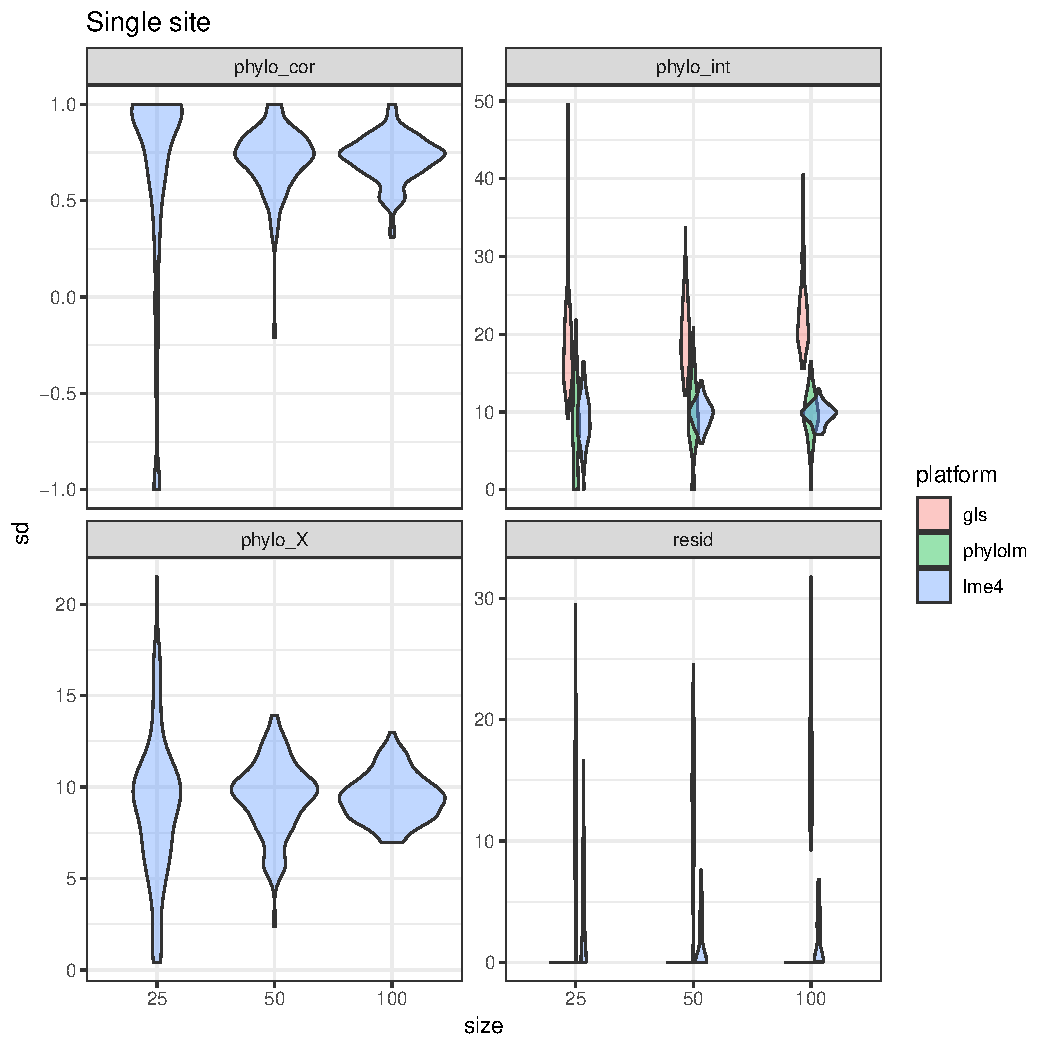
\includegraphics[scale=0.8,page=1]{./git_push/plot.Rout.pdf}
  \caption{New}
\label{ssplot}
\end{figure}
\end{center}


\begin{center}
\begin{figure}[h]
  \includegraphics[scale=0.8,page=2]{./git_push/plot.Rout.pdf}
  \caption{New}
\label{ssplot}
\end{figure}
\end{center}


\begin{center}
\begin{figure}[h]
  \includegraphics[scale=0.8,page=3]{./git_push/plot.Rout.pdf}
  \caption{New}
\label{ssplot}
\end{figure}
\end{center}


\bmb{Need to think a little harder about the important points/order here (might be time to do the exercise where you take the results and boil them back down to short bullet points, in order to figure out whether you've said the important stuff, in the right order). Maybe lead by saying that all platforms give similar answers - to the extent that they are fitting the same statistical model (this might even be emphasized/explained above, in Methods). Am I correct in believing that phylolm=\pkg{lme4} but without intercept/slope correlation, and gls is additionally missing random slopes?}

\bmb{add refs to figures \ldots}

% \begin{itemize}
% \item{full model provides good estimates (except for correlation)}
% \item{reduced models try to fit with whatever parameters they have available (over-estimates the simulation parameters)}
% \item{no slope vs slope}
% \item{no correlation vs correlation}
% \item{as size/data/number of species increase, the parameter estimates gets better}
% \item{single site models are fast}
% \item{estimates gets closer to simulation parameter as number of species increase}
% \item{lme4/tmb are fast, everything else is slow for multiple sites}
% \end{itemize}

The full single site model using phyloglmm (which matches the single simulation model that incorporates phylogenetic intercept, slope and correlation) provides good estimates for all parameters except for random correlation parameter ($\sigma_{phy_{int},phy_{slope}}$). 
Fixed effect parameters ($\beta_0$ and $\beta_1$) estimates approaches nominal coverage as number of species increases.
\mli{go back and define coverage and how its used}

In general, models that cannot match the simulation model (PGLM and PGLS) will try to fit the data with the parameters available. 
PGLM (which lacks the phylogenetic slope parameter) provides reasonable good estimates for phylogenetic intercept parameter ($\sigma_{phy_{int}}$) but overestimates the residual/observation standard deviation. 
$\beta_0$ estimates slightly undercover the nominal coverage (90\% with 100 species) and have a bad coverage ($<$ 60\%) for the fixed slope parameter.
PGLS, with only one parameter available, confounds all variations (phylogenetic intercept, slope and residual variation) into the single parameter (phylogenetic intercept), resulting in overestimating the phylogenetic intercept as well as large RMSE and overcovering for $\beta_0$, and bad estimates for $\beta_1$. 
\mli{double check this, what happens when X is also phylogenetically correlated?}

% \bmb{(2) please define ``robustness'' -- usually means lack of sensitivity to model.  Are you talking about the variance of the estimates? I'd prefer not to use ``robust'' in a non-standard way if possible (2) what are small/medium/large? I see that $n=\{20,100,500\}$ and $m=\{1,20\}$, but not sure how these match up to ``small'', ``medium'', ``large''; is Figure 1 all $m=1$? Might be worth just labeling by $n=??$ rather than using small/medium/large}
% It is unclear how different levels of phylogenetic signal are being confounded under the error free (without tip variation) assumption for the PGLS models.
% \bmb{can we figure this out, even in an empirical/crude way??? it's tough to have results without knowing the true value they're aiming for ...}


\begin{center}
\begin{figure}[h]
  \includegraphics[scale=0.8,page=4]{./git_push/plot.Rout.pdf}
  \caption{new}
\end{figure}
\end{center}


\begin{center}
\begin{figure}[h]
  \includegraphics[scale=0.8,page=6]{./git_push/plot.Rout.pdf}
  \caption{new}
\end{figure}
\end{center}


\begin{center}
\begin{figure}[h]
  \includegraphics[scale=0.8,page=7]{./git_push/plot.Rout.pdf}
  \caption{new}
\end{figure}
\end{center}


Multiple site fits on the other hand are a lot more similar across platforms (as there are less deviates between the fitted and simulation model) compared to the single site fits.
Similar to the single site fits, phyloglmm which matches the simulation model provides good estimates for all parameters except for the random correlation parameter ($\sigma_{sp_{int,slope}}$).
\mli{either keep it or take it out, because  will affect other parameters}
The lack of correlation in \pkg{phyr}'s statistical models does not appear to have a large effect on its ability to estimate other parameters, whereas \pkg{pez} underestimates (lower estimates) many parameters.  
\bmb{Can you identify the extreme cases in \pkg{lme4}'s estimate? Are these singular models? Would they be diagnosable? Can you say anything about when the assumption of independence of slope and intercept \textbf{would} be a problem? (If you can think of such a scenario, you could run sims for one such example - don't need to go into great detail, but being able to say that you confirmed that it's a problem in such-and-such a case would be important.)}
\mli{save it for random slope discussion}

However, despite the similarities of parameter estimates across platforms/methods for the multiple sites simulations fits, the efficiency (measured by computational speed) are different across playforms/methods and sample size.
For example, the median time for \pkg{lme4} to fit 50/100 species model takes $~$ 50/100 seconds versus $~$ 200/2000 seconds for \pkg{pez} and \pkg{phyr}. 
Lastly, it takes $~$ 2000 seconds for lme4 to fit 1000 species model and it was not practical for \pkg{pez} and \pkg{phyr} to fit 1000 species models where the computational speed did not scale linearly with sample size 25/50/100.
\mli{put a lower bound to give up}

\bmb{Can you put a lower bound on \pkg{pez}'s computation time? How long did you take to give up? How does it scale? can you either figure out from first principles
  or (easier) do a brute-force series of increasing sample size and
  compute a log-log regression of time vs sample size to find the
  approximate power?}

We used our method and fitted the full model of the dune meadow data recently used with \pkg{pez} \cite{li2017canfun}. 
We have obtained identical results for fix and random effect estimates and approximately 120 times faster compared to \pkg{pez}. 
Codes for fitting dune meadow analysis using \pkg{lme4} and \pkg{pez} are provided in the supplements. 

\newpage

\section{Discussion}


% \bmb{say something about the implications of this [e.g. good enough for getting an overall impression of phylog. whatever-it-is but not enough for detailed description/inference about the evolutionary process?] (or maybe that should be saved for the Discussion?)}

The evolutionary model simulations presented in this paper are an oversimplification of real evolutionary processes in nature, but it is analogous to how researchers fit models to study complicated systems (as it is impossible to create a model to "match" the complexities of nature).
We have fitted models using different platforms/methods that best match the simulation models. 
Models that cannot match the simulation (full) model are expected to underperform; it is important to understand the limitations and performance of these simpler models/assumptions that are restricted by the commonly used methods available.
Using models that include some form of phylogenetic variation and residual variation is necessary to \mli{correctly/robustly?} detect evolutionary process.

\subsection{Process and residual (observation) variabilities and confoundings}

Process and observation errors are highly confounded in phylogenetic regression if it is not handled correctly. 
The effects of models that include both process and residual variations (i.e. PGLMM, PGLM) instead of the less realistic model that assumes variation due to evolution and zero observation (PGLS) was large. 
% In particular, models that did not include residual variation tended to over-estimate the amount of variability in the evolutionary process. 
Thus, for single measurement per species model, any method that can account for at least two sources of variation (one for the residual variance, and at least one for the process variation) will be sufficient to a first approximation (i.e. Pagel's $\lambda$, Blomberg's $K$).
However, if multiple measurements/observations are considered/allowed per species, then using methods such as Pagel's $\lambda$ can potentially incorrectly estimate the amount of phylogenetic process by substituting tip variation with residual variation. 

\mli{this is specifically targeting boettiger's critque on Pagel's lambda.
https://www.carlboettiger.info/2013/10/11/is-it-time-to-retire-pagels-lambda.html
The difference between the two figures is what it thinks the "tip" variation is. For the second plot, if we treat the sister taxas as "multiple" observation with some observation error on it, then you will get back to the first plot.}

\bmb{again, we/you need to think carefully about what these coarse measures are good for; just avoiding mis-estimating the strength of trait/trait or trait/environment parameters? Is it worth doing some sims on that, or do we basically believe if the total amount of phylogenetic signal is correctly assessed, that we get the right answer for the trait effect? Is \cite{schielzeth2009conclusions} relevant/a useful analogy? (You cite it below, but there are two separate questions: (1) whether including random slopes gives us more insight into evol processes; (2) whether omitting random slopes gives us bad answers even when we're not interested in them.) Worth citing/discussing \cite{uyeda2018rethinking} (as an example of even deeper analysis of evolutionary processes, beyond BM etc.)?}

\subsection{Random Slopes}

\bmb{I think you need a lot more here; what does a random slopes model mean? You have one sentence that says ``people should be thinking about random slopes''. Then you talk about correlation (which is a much more subtle/less important issue, I think).}
In classic GLMM (without phylogenetic relationships), random slopes models are not always appropriate, but they are relevant over a wider range of scenarios than people are currently thinking about \cite{schielzeth2008conclusions, cleasby2015quantifying,ord2010adaptation}.
When analyzing relationships among species between traits and environmental variables, it is entirely plausible that change in effect of predictor variables have on traits are changing in a phylogenetically correlated way.
In fact, it is easier to interpret random slopes in the evolutionary process context (i.e, are size of different species phylogenetically correlated, or growth rate through time of different species phylogenetically correlated?)
\mli{I like to think of it in a longitudinal setting of observing plant length/height. At time zero, they are all still seeds, one can imagine the growth rate are different plant species grow in a phylogenetically correlated way (similar species have similar growth rates).}
It may be easier to simplify the phylogenetic relationships (at the random slopes level) and think about the random-slopes model in a strictly hierarchical setting (i.e., estimating different slopes for each family, or taxon \cite{bunnefeld2012island}) - the PGLMM collapses to a standard random-slopes model. 
Users should be aware of two important questions when fitting random-slope models: How much data do we need in order to practically estimate the random slopes? and Are we making a mistake by ignoring random slopes \cite{schielzeth2008conclusions}? 
However, in the PGLMM context, as long as there's variation in the predictor among tips, there will be variation among taxa at some level, so random-slopes models will (almost always) be \emph{theoretically} identifiable.


\subsection{Extension and alternatives}

Our analysis covers the classical phylogenetic comparative methods (i.e. phylogenetic least squares, linear and mixed models).
Even within the scope there is additional room for exploration we neglected, such as exploring phylogenetic multivariate response models, non-BM evolution processes (such as Ornstein-Uhlenbeck (OU) process which accounts for both selection and drift processes \cite{butler2004phylogenetic}), Bayesian approaches \cite{hadfield2010general}.
More broadly, the simple independence error approach we developed here offers a more efficient and mathematical equivalent way to do Brownian motion evolution process phylogenetic comparative analysis. 
This approach can in principle be combined flexibly with the state of the art phylogenetic mixed models using platforms that supports independent latent variables such as \pkg{MCMCglmm} \cite{hadfield2010mcmc}; a widely used Bayesian approach to PGLMM.
However, in principle just like GLMM and most statistically models, users should be aware the amount of data they have and the complexity of the model they want to fit (i.e. What should we do when we don't have enough data? Should we use a complex model and overfit \cite{barr2013random}, the right balance of complexity and data \cite{baayen2008mixed} or possibility of Bayesian approaches \cite{hadfield2010mcmc}).
More importantly, this implementation in \pkg{lme4} allows users to fit phylogenetic mixed models to the fullest ( that other frequentist platforms lack of (i.e. large data, unbalanced species observations, complex random effects) and explore new ideas.


\section{Conclusion}

We have presented a simple approach to fit phylogenetic mixed models that is both more efficient and statistically equivalent approach and comparison of classical PCM to simulated data. 
First, this new approach is magnitudes faster compared to existing phylogenetic mixed models without losing robustness/accuracy and can easily combined with any statistically mixed model framework. 
Last and most importantly, it is more flexible in fitting large phylogenies, large volume of data, unbalanced data sets, and complex random effects such as slope correlations.

\newpage

\section{Supplements -- translation}

$1 \mid Sp_{phylo}$, $0 + X_{E} \mid Sp_{phylo}$ and $X_{E} \mid Sp_{phylo}$ means phylogenetically related have similar response,   

\begin{tabularx}{\textwidth}{|l|X|X|}
\hline
Formula & Statistics & Biology \\
\hline
$1 \mid Sp$ &
random species intercept; variation within species in mean response across all factors &
variation of how species respond \\
\hline

$0 + X_{E} \mid Sp$ &
random slope of environment factor within species; variation in coefficient within species for the environmental factor &
variation of how species respond to the same environmental factor \\
\hline

$1 + X_{E} \mid Sp$ &
random slope of environmental factor within species with correlated intercept; variation in coefficient within species for the environmental factor with correlated mean response across all other factors &
variation of how species respond in the same environmental factors and the correlation of the variation of how they respond in general \\
\hline

$1 \mid Site:Sp $ &
random variation in intercept among species within sites &
variation of how species respond within sites \\
\hline

$1 | Sp_{Phylo} $ &
variation among species in mean response across all factors demonstrate phylogenetic signal &
phylogenetically related species respond similarly \\
\hline

$0 + X_{E} \mid Sp_{Phylo}$ &
variation among species for environmental factors demonstrate phylogenetic signal &
phylogenetically related species respond similar (share common response) to the same environmental factor \\
\hline
\end{tabularx}
            
            
            
            
            
                                                              
